\documentclass{beamer}

\usepackage{graphicx}
\usepackage{booktabs}
\usetheme{CambridgeUS}

\title{CS 490: Goodreads Genre Network}
\subtitle{Analysis of Book Similarity Networks}
\author{Shayne Tieman}
\date{April 2026}

\begin{document}

  \begin{frame}
    \titlepage
  \end{frame}

  %% slide 1: Introduction
  \begin{frame}
    \fontsize{10}{12}\selectfont
    \fontsize{12}{14}\selectfont
    \textbf{Introduction}
    
    \vspace{0.5cm}
    \textbf{Goal}: Build a book recommendation network by clustering Goodreads books based on genre similarity rather than Goodreads' native categorization
    
    \vspace{0.5cm}
    \textbf{Methods Used}:
    \begin{itemize}
      \item Jaccard similarity for genre matching (weight: 0.6)
      \item Number of ratings similarity (log-scaled, weight: 0.2)
      \item Rating similarity (1 - |r1-r2| / 1.0, weight: 0.2)
      \item Combined: 0.6 $\times$ genre + 0.2 $\times$ num\_ratings + 0.2 $\times$ rating
      \item Threshold = 0.7 for edge creation
    \end{itemize}
    
    \vspace{0.5cm}
    \textbf{Data}: ~10,000 books from Kaggle datasets
  \end{frame}

  %% slide 2: Basic Network Statistics
  \begin{frame}
    \fontsize{10}{12}\selectfont
    \textbf{Basic Network Statistics}
    
    \vspace{0.3cm}
    \begin{table}
      \centering
      \fontsize{10}{12}\selectfont
      \begin{tabular}{lcc}
        \toprule
        Metric & Goodreads Network & ER Network \\
        \midrule
        Nodes & 10,000 & 10,000 \\
        Edges & 175,890 & 100,000 \\
        Density & 0.0035 & 0.0020 \\
        Avg Degree & 35.18 & 20.00 \\
        Max Degree & 436 & 41 \\
        \bottomrule
      \end{tabular}
    \end{table}
  \end{frame}

  %% slide 3: Random Graph Comparison
  \begin{frame}
    \fontsize{10}{12}\selectfont
    \textbf{Random Graph (Erd\^{o}s-R\'{e}nyi)}
    
    \vspace{0.3cm}
    Generated ER random graph with same n,m as our network
    
    \vspace{0.3cm}
    \begin{center}
      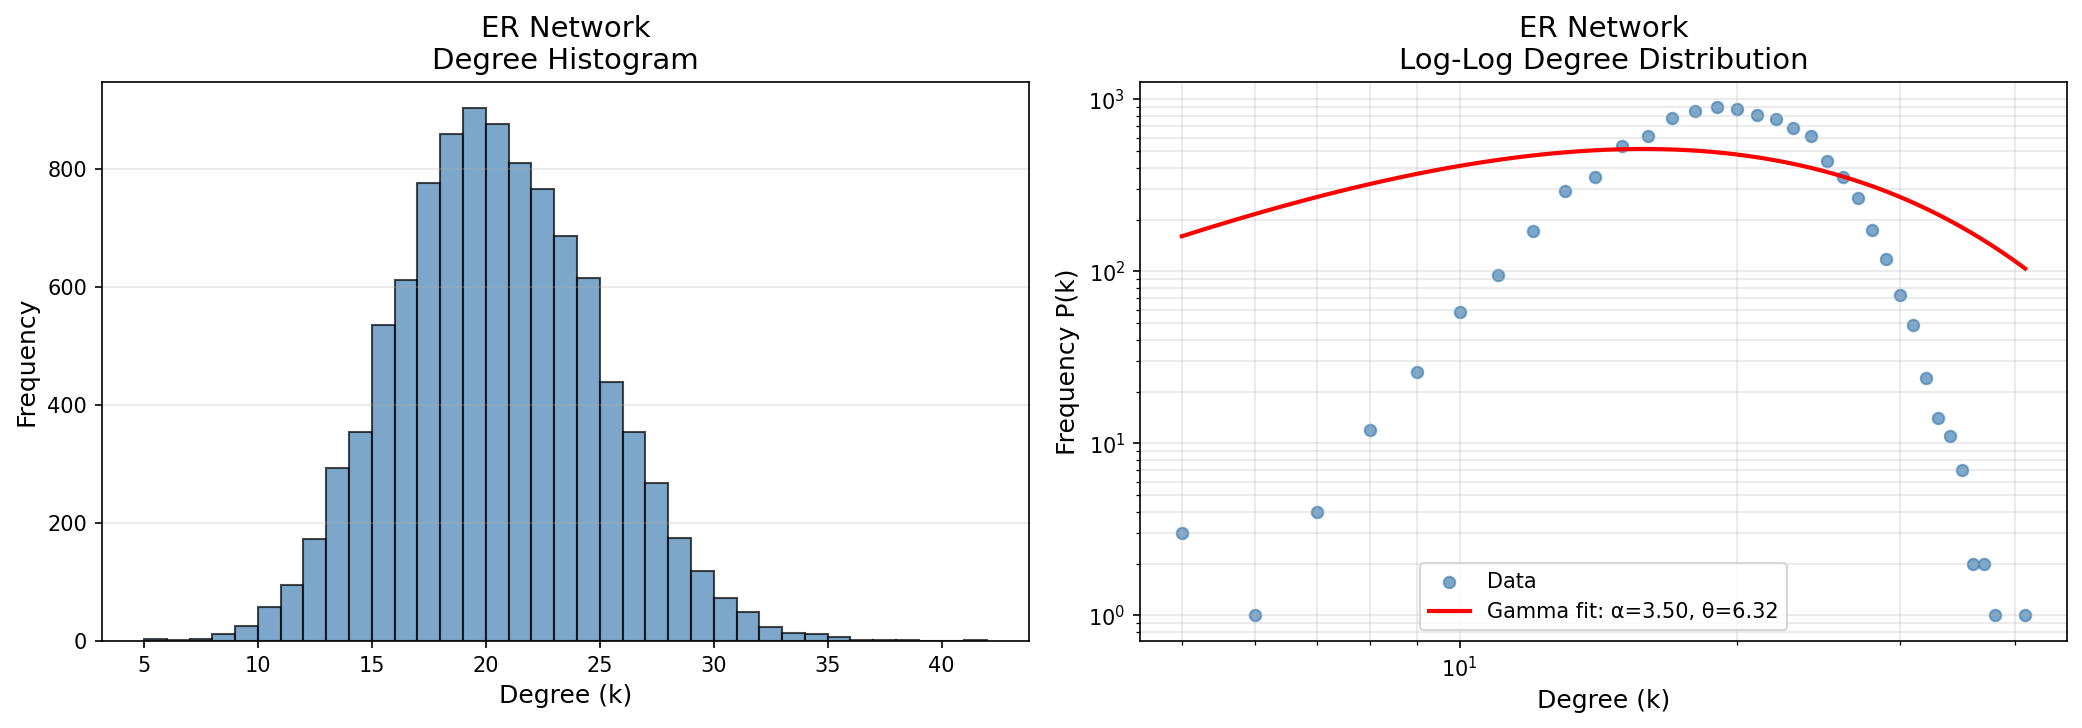
\includegraphics[width=0.85\linewidth]{../img/ER.png}
    \end{center}
    
    \vspace{0.3cm}
    \begin{table}
      \centering
      \fontsize{9}{11}\selectfont
      \begin{tabular}{lcc}
        \toprule
        Metric & Goodreads Network & ER Network \\
        \midrule
        Clustering Coeff & 0.4137 & 0.0020 \\
        Modularity (Greedy) & 0.7103 & 0.1740 \\
        Modularity (Louvain) & 0.7686 & 0.1795 \\
        Assortativity & 0.7801 & 0.0033 \\
        \bottomrule
      \end{tabular}
    \end{table}
  \end{frame}

  %% slide 4: Gephi Visualization
  \begin{frame}
    \fontsize{10}{12}\selectfont
    \textbf{Gephi Graph Visualization}
    
    \vspace{0.3cm}
    \begin{center}
      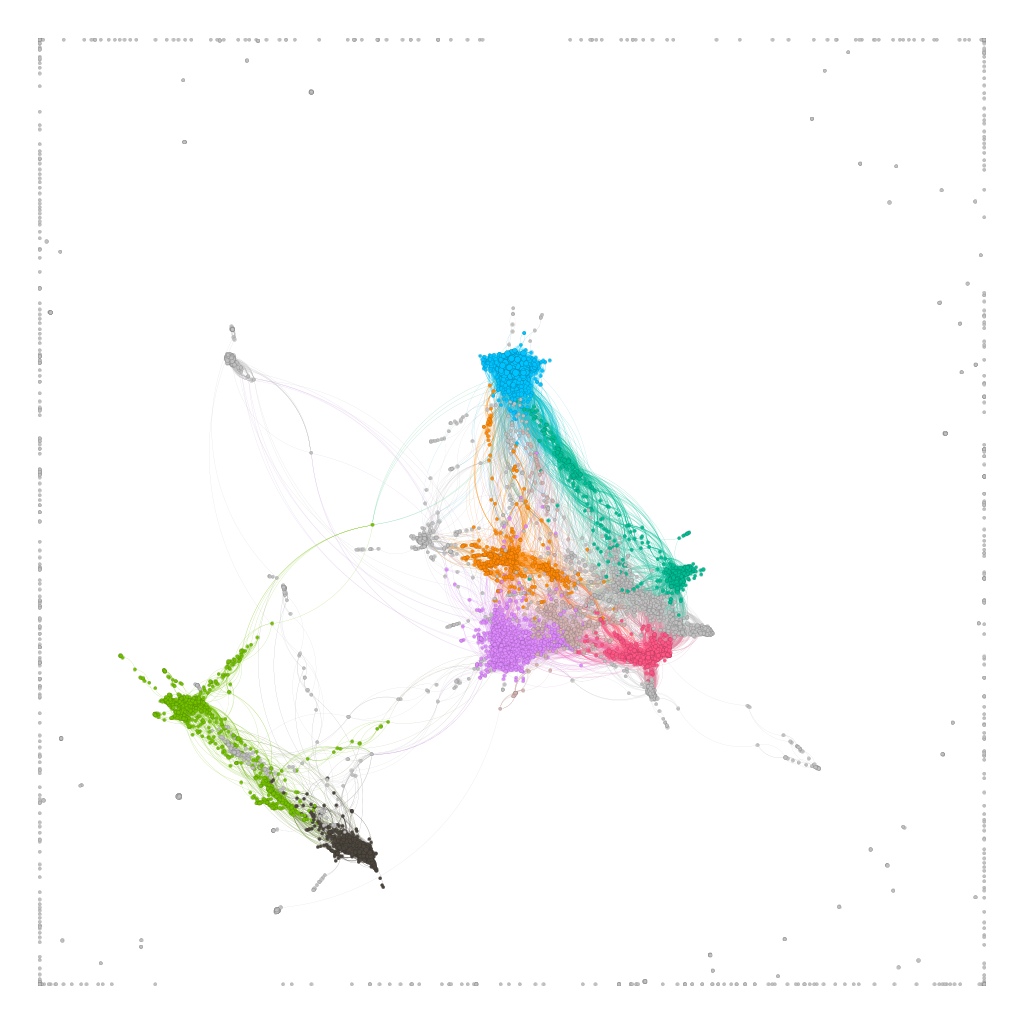
\includegraphics[width=0.7\linewidth,height=0.5\textheight,keepaspectratio]{../img/gephi.png}
    \end{center}
    
    \vspace{0.3cm}
    \textbf{Color coding}: By community / genre cluster
    
    \textbf{Size}: Node size by degree
  \end{frame}

  %% slide 5: Degree Distribution
  \begin{frame}
    \fontsize{10}{12}\selectfont
    \textbf{Degree Distribution}
    
    \vspace{0.3cm}
    \begin{center}
      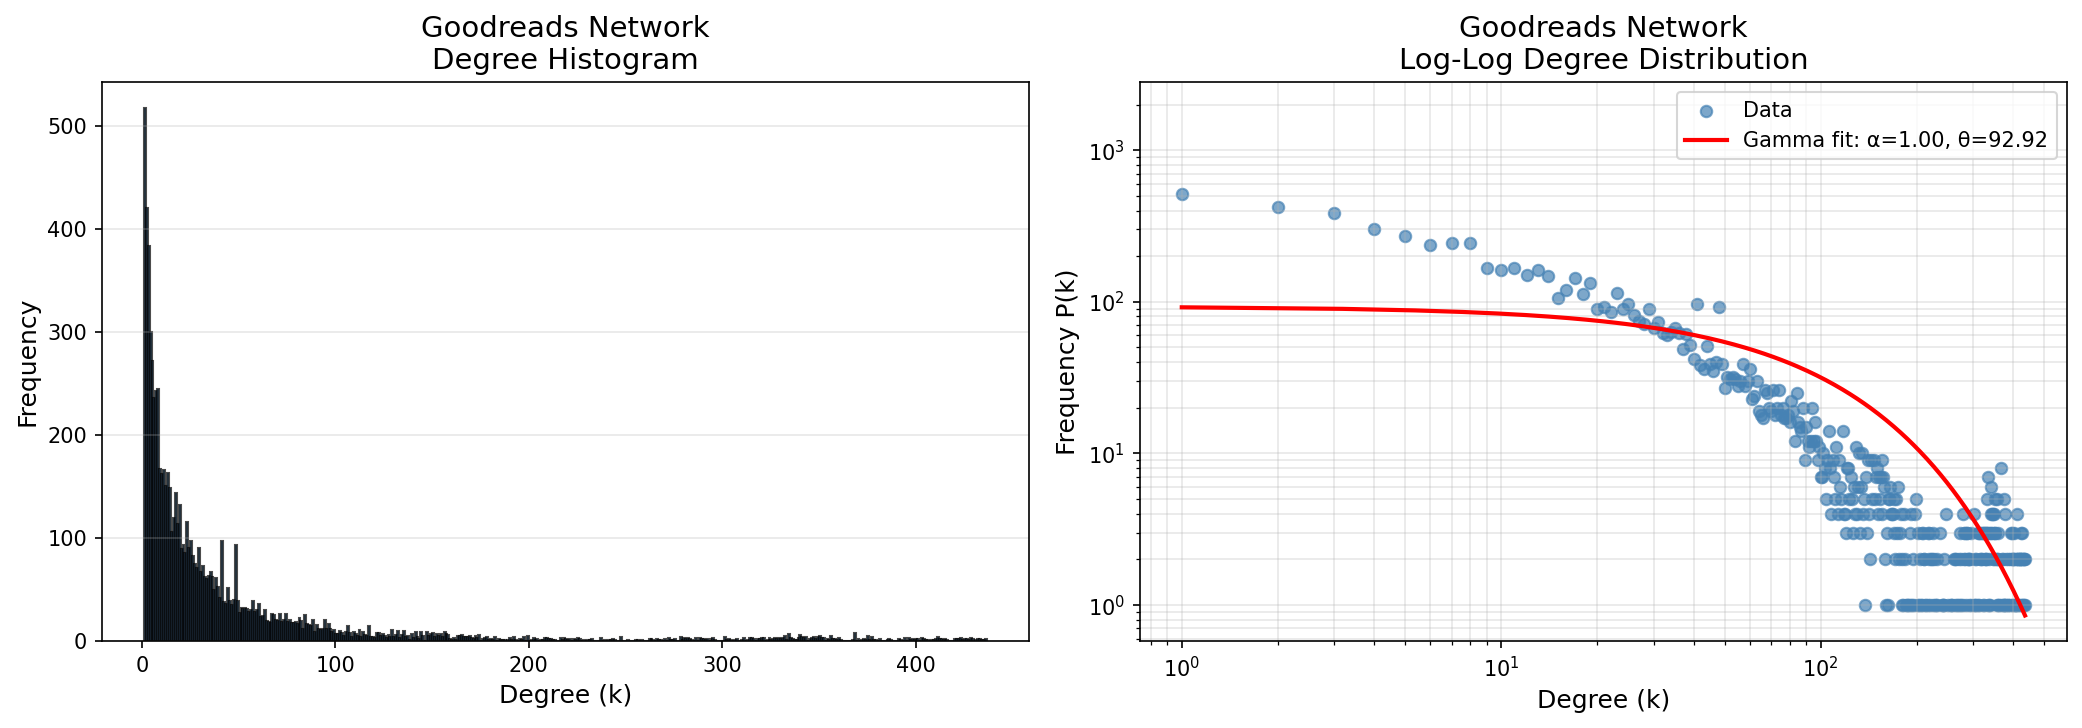
\includegraphics[width=0.9\linewidth]{../img/degree_distribution.png}
    \end{center}
    
    \vspace{0.3cm}
    \textbf{Key observations}:
    \begin{itemize}
      \item Heavy-tailed distribution (scale-free properties)
      \item Few highly connected ``hub'' books connect many genres
      \item Average degree: 35.18 vs ER average: 20.00
    \end{itemize}
  \end{frame}

  %% slide 6: Graph Analysis
  \begin{frame}
    \fontsize{10}{12}\selectfont
    \textbf{Graph Analysis Methods}
    
    \vspace{0.5cm}
    \textbf{Statistics Computed}:
    \begin{itemize}
      \item Nodes, Edges, Density
      \item Degree distribution (mean, variance, max)
      \item Clustering coefficient
      \item Degree assortativity
    \end{itemize}
    
    \vspace{0.3cm}
    \textbf{Community Detection}:
    \begin{itemize}
      \item Greedy Modularity
      \item Louvain method
      \item Label Propagation
    \end{itemize}
    
    \vspace{0.3cm}
    \textit{All computed using NetworkX library}
  \end{frame}

  %% slide 7: Comparison with Original
  \begin{frame}
    \fontsize{10}{12}\selectfont
    \textbf{Comparison with Original Goodreads Network}
    
    \vspace{0.3cm}
    Our approach vs Goodreads' native genre categorization:
    
    \vspace{0.3cm}
    \begin{table}
      \centering
      \fontsize{10}{12}\selectfont
      \begin{tabular}{lcc}
        \toprule
        Feature & Our Network & Goodreads \\
        \midrule
        Clustering basis & Genre + Num\_Ratings + Rating & Single genre \\
        Similarity metric & Jaccard + log(popularity) + Rating & Binary \\
        Weights & 0.6 + 0.2 + 0.2 & Implicit \\
        Edge threshold & 0.7 & Implicit \\
        Community detection & Yes (Q=0.77) & No \\
        \bottomrule
      \end{tabular}
    \end{table}
    
    \vspace{0.3cm}
    \textit{Note: Need to research Goodreads' actual method}
  \end{frame}

  %% slide 8: Clustering Explained
  \begin{frame}
    \fontsize{10}{12}\selectfont
    \textbf{Clustering Coefficient Explained}
    
    \vspace{0.5cm}
    Measures degree of transitivity in the network
    
    \vspace{0.3cm}
    $C = \frac{3 \times \text{triangles}}{\text{connected\_triples}}$
    
    \vspace{0.5cm}
    \textbf{Interpretation}:
    \begin{itemize}
      \item $C \approx 0$: Random network
      \item $C > 0.01$: Some clustering (our expected result)
      \item $C > 0.1$: Highly clustered
    \end{itemize}
  \end{frame}

  %% slide 9: Clustering Methods
  \begin{frame}
    \fontsize{10}{12}\selectfont
    \textbf{Community Detection Methods Comparison}
    
    \vspace{0.3cm}
    \begin{table}
      \centering
      \fontsize{10}{12}\selectfont
      \begin{tabular}{lccc}
        \toprule
        Method & Communities & Modularity & Runtime \\
        \midrule
        Greedy Modularity & 2,101 & 0.7103 & ~56s \\
        Louvain & 2,080 & 0.7686 & ~4s \\
        Label Propagation & 2,327 & 0.7383 & ~2s \\
        \bottomrule
      \end{tabular}
    \end{table}
    
    \vspace{0.5cm}
    \textbf{Quality metric}: Modularity $Q \in [-0.5, 1]$
    \begin{itemize}
      \item $Q > 0.3$: Significant community structure
      \item Higher = better partitioning
    \end{itemize}
  \end{frame}

  %% slide 10: Interpretation
  \begin{frame}
    \fontsize{10}{12}\selectfont
    \textbf{Interpretation of Results}
    
    \vspace{0.5cm}
    \textbf{Key Findings}:
    \begin{enumerate}
      \item Books cluster naturally by genre $\rightarrow$ strong modularity
      \item Degree distribution follows power-law $\rightarrow$ scale-free
      \item Comparison with ER shows significant structure
    \end{enumerate}
    
    \vspace{0.5cm}
    \textbf{Implications}:
    \begin{itemize}
      \item Genre-based similarity captures real book relationships
      \item Network analysis reveals book communities beyond single-genre labels
      \item Potential for better recommendation systems
    \end{itemize}
  \end{frame}

  %% slide 12: The End
  \begin{frame}
    \centering
    \fontsize{14}{16}\selectfont
    \textbf{Questions?}
    
    \vspace{1cm}
    \fontsize{12}{14}\selectfont
    Code: github.com/zaigiaz/goodreads-network
    
    \vspace{0.5cm}
    \textit{Run: python data\_analysis.py --file 1 --clustering --communities --assortativity}
  \end{frame}

\end{document}
